\documentclass[11pt]{scrartcl}
\usepackage{graphicx}
\graphicspath{{./}}
\usepackage[sexy]{evan}
\usepackage[normalem]{ulem}
\usepackage{hyperref}
\usepackage{mathtools}
\hypersetup{
    colorlinks=true,
    linkcolor=blue,
    filecolor=magenta,      
    urlcolor=cyan,
    pdfpagemode=FullScreen,
    }

\renewcommand{\dangle}{\measuredangle}

\renewcommand{\baselinestretch}{1.5}

\addtolength{\oddsidemargin}{-0.4in}
\addtolength{\evensidemargin}{-0.4in}
\addtolength{\textwidth}{0.8in}
% \addtolength{\topmargin}{-0.2in}
% \addtolength{\textheight}{1in} 


\setlength{\parindent}{0pt}

\usepackage{pgfplots}
\pgfplotsset{compat=1.15}
\usepackage{mathrsfs}
\usetikzlibrary{arrows}

\title{Combinatorial Games dan Invarian - Soal Latihan}
\author{Azzam (IG: haxuv.world)}
\date{Kamis, 25 Januari 2024}

\begin{document}
\maketitle
% https://www.math.uwaterloo.ca/~snew/Contests/ProblemSessions/Problems2016/Lesson0soln.pdf
% 30 soal kombin
% Arthur Engel
% Soberon
\section{Invarian dan Monovarian}
\begin{enumerate}
\item (OSN 2015) Albert, Bernard dan Cheryl sedang bermain kelereng. Di awal permainan masing- masing membawa 5 kelereng merah, 7 kelereng hijau dan 13 kelereng biru, sedangkan di kotak kelereng ada tak berhingga banyaknya kelereng. Pada satu langkah setiap anak diberi kebebasan membuang dua kelereng yang berbeda warna, kemudian menggantinya dengan dua kelereng dengan warna ketiga. Sebagai contoh, satu kelereng hijau dan satu kelereng merah dibuang, kemudian dua kelereng biru diambil dari kotak. Setelah serangkaian langkah (banyaknya langkah yang dilakukan masing-masing anak boleh berbeda) terjadilah percakapan berikut.
    \begin{itemize}
        \item Albert : “Saya hanya membawa kelereng berwarna merah.”
        \item Bernard : “Saya hanya membawa kelereng berwarna biru.”
        \item Cheryl : “Saya hanya membawa kelereng berwarna hijau.”
    \end{itemize}
    Siapa sajakah yang pasti berkata bohong?

\item (OSN 2016) Lima buah kotak disusun secara melingkar, dengan satu kotak berisi satu bola dan kotak-kotak lainnya kosong. Ada dua operasi yang diizinkan untuk dilakukan terhadap kotak dan bola ini:
    \begin{enumerate}[(i)]
        \item  satu bola dari suatu kotak tak kosong, lalu tambahkan satu bola ke masing-masing dua kotak tetangganya (yang berada di kiri dan kanan kotak yang diambil bolanya)
        \item Ambil satu bola dari suatu kotak tak kosong, lalu masukkan bola tersebut ke salah satu kotak kosong di sebelah kotak tersebut.
    \end{enumerate}
    Mungkinkah pada akhirnya, setiap kotak berisi tepat $17^{5^{2016}}$ bola?

\item (OSN 2010) Sebanyak $m$ orang anak laki-laki dan $n$ orang anak perempuan ($m > n$) duduk mengelilingi meja bundar diawasi oleh seorang guru, dan mereka melakukan sebuah permainan sebagai berikut. Mula-mula sang guru menunjuk seorang anak laki-laki untuk memulai permainan. Anak laki-laki tersebut meletakkan sekeping uang logam di atas meja. Kemudian bergiliran searah jarum jam, setiap anak melakukan gilirannya masing-masing. Jika anak tersebut laki-laki, ia menambahkan sekeping uang logam ke tumpukan di atas meja, dan jika anak tersebut perempuan, ia mengambil sekeping uang logam dari tumpukan tersebut. Jika tumpukan di atas meja habis, maka permainan berakhir saat itu juga. Perhatikan bahwa tergantung siapa yang ditunjuk oleh sang guru untuk memulai langkah pertama, maka permainan tersebut bisa cepat berakhir, atau bisa saja berlangsung paling sedikit $1$ putaran penuh.
Jika sang guru menginginkan agar permainan tersebut berlangsung paling sedikit $1$ putaran penuh, ada berapa pilihan anak laki-laki yang dapat beliau tunjuk untuk memulai?

\item Show that if 25 people play in a ping pong tournament then, at the end of the tournament, the number of people who played an even number of games is odd.

\item Show that in a house with 25 rooms, if every room has an odd number of doors then there must be an odd number of doors along the outside wall of the house.

\item Find the minimum number of breaks required to break an $m \times n$ bar of chocolate into $1 \times 1$ squares.

\item We begin with the numbers $1, 2, 3, \ldots , 50$ written on the blackboard. At each step we can erase any two of the numbers $a$ and $b$ and then write down the number $|a-b|$. We continue until one number remains. Determine whether this final number could be equal to $10$.

\item Let $A$ be a matrix with integral entries. Show that there exist diagonal matrices $B$ and $C$ whose diagonal entries are all $\pm1$ such that in the matrix $BAC$ the sum of the entries in each row and in each column is non-negative.

\item Determine whether it is possible to tile a $10 \times 10$ square floor using $1 \times 4$ rectangular tiles.

\item We try to tile a $k \times l$ rectangular floor using some $2 \times 2$ square tiles and some $1 \times 4$ rectangular tiles. Show that if it is possible to tile the floor using $m$ of the square tiles and $n$ of the rectangular tiles, then it is not possible to tile the floor using $(m + 1)$ of the square tiles and $(n - 1)$ of the rectangular tiles.

\item Show that when a $6 \times 6$ square floor is tiled using $1 \times 2$ rectangular tiles, there is always a straight line which crosses the floor without cutting through any of the tiles.

\item Initially, $9$ of the $100$ squares in a $10 \times 10$ grid are infected. During each unit time interval, each square which has $2$ or more infected neighbours (a neighbour being a square which shares an edge) also becomes infected. Determine whether it is possible that all $100$ squares will eventually become infected.

\item Initially, $4$ chips are placed at the point $(0, 0)$. At each step we can remove one chip from some point $(a, b)$ and replace it with $2$ chips, one at the point $(a + 1, b)$ and the other at $(a, b + 1)$. Show that, after finitely many steps, there will always be some point with at least two chips sitting on it.


% \item There are three piles with $n$ tokens each. In every step we are allowed to choose two piles, take one token from each of those two piles and add a token to the third pile. Using these moves, is it possible to end up having only one token?

\item Let $n$ be a positive integer and consider the ordered list $(1, 2, 3,...,n)$. In each step we are allowed to take two different numbers in the list and swap them. Is it possible to obtain the original list after exactly $2009$ steps?

\item (IMO 2011) Let $S$ be a finite set of at least two points in the plane. Assume that no three points of $S$ are collinear. A windmill is a process that starts with a line $l$ going through a single point $P \in S$. The line rotates clockwise about the pivot $P$ until the first time that the line meets some other point belonging to $S$. This point, $Q$, takes over as the new pivot, and the line now rotates clockwise about $Q$, until it meets a point of $S$. This process continues indefinitely. Show that we can choose a point $P$ in $S$ and a line $l$ going through $P$ such that the resulting windmill uses each point of $S$ infinitely many times.

\item $23$ friends want to play soccer. For this they choose a referee and the others split into two teams of $11$ persons each. They want to do this so that the total weight of each team is the same. We know that they all have integer weights and that, regardless of who is the referee, it is possible to make the two teams. Prove that they all have the same weight.

\item (IMO 1986) We assign an integer to each vertex of a regular pentagon, so that the sum of all is positive. If three consecutive vertices have assigned numbers $x$, $y$, $z$, respectively, and $y < 0$, we are allowed to change the numbers $(x,y,z)$ to $(x + y,-y,z + y)$. This transformation is made as long as one of the numbers is negative. Decide if this process always comes to an end.


\end{enumerate}

\section{Coloring}
\begin{enumerate}[resume]
\item Is it possible to cover a $10 \times 10$ board with the following pieces without them overlapping? Note: The pieces can be flipped and turned.
\begin{figure}[h]
    \centering
    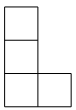
\includegraphics{Kombin/Game-Invariant/tetromino-L.png}
\end{figure}

\item On a $9 \times 9$ board $65$ insects are placed in the centers of some of the squares. The insects start moving at the same time and speed to a square that shares a side with the one they were in. When they reach the center of that square, they make a $90$ degrees turn and keep walking (without leaving the board). Prove that at some moment of time there are two insects in the same square. Note: When they turn it can be either to the right or to the left.

\item (IMO shortlist 2002) A $(2n - 1) \times (2n - 1)$ board is going to be tiled with pieces of the type as shown. Prove that at least $4n - 1$ of the first type will be used.
\begin{figure}[h]
    \centering
    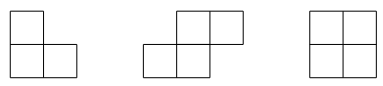
\includegraphics{Kombin/Game-Invariant/IMOSL2002Domino.png}
\end{figure}

\item
    2023 koin akan diletakkan pada papan berukuran $n \times n$ sedemikian sehingga selisih banyaknya koin pada setiap 2 persegi yang bertetangga adalah 1. Jika 2 persegi disebut bertetangga apabila mereka mempunyai atau berbagi satu sisi yang sama, carilah nilai $n$ terbesar yang mungkin.


\item
    Apakah mungkin untuk berjalan pada taman yang menyerupai papan catur $8 \times 8$ sehingga anda hanya bisa berjalan melewati setiap kotak $1 \times 1$ tepat sekali dengan kotak awal dan kotak akhir perjalanan tersebut berada pada ujung-ujung (corner) yang saling berlawanan? (Anda hanya diperbolehkan berjalan ke kotak yang bertetangga atau tepat bersebelahan dari kotak anda sekarang).


\item
    Diketahui bahwa delapan persegi panjang berukuran $1 \times 3$ dan satu kotak berukuran $1 \times 1$ menutup papan berukuran $5 \times 5$. Tunjukkan bahwa kotak berukuran $1 \times 1$ tersebut harus berada di tengah papan. (persegi panjang berukuran $1 \times 3$ dan $3 \times 1$ dianggap sama)


\item
    Dapatkah papan $8\times8$ ditutupi dengan lima belas persegi panjang $1\times4$ dan satu buah persegi $2\times2$ tanpa tumpang tindih?


\item
    Misalkan $m,n > 2$ adalah bilangan bulat. Warnai setiap persegi $1\times1$ dari papan $m\times n$ dengan warna hitam atau putih (tetapi tidak keduanya). Jika dua persegi $1\times1$ yang tepat saling bersebelahan memiliki warna yang berbeda, maka sebut pasangan persegi ini sebagai pasangan "roman". Definisikan $S$ menjadi jumlah pasangan roman di papan $m\times n$. Buktikan bahwa genap atau ganjilnya $S$ hanya tergantung pada persegi $1\times1$ pada pinggiran papan selain 4 persegi $1\times1$ di ujung-ujung sudut papan.


\item
    Terdapat 1004 titik yang berbeda pada sebuah bidang. Hubungkan setiap pasang titik tersebut dan tandai titik tengah dari segmen garis ini dengan warna hitam. Buktikan bahwa terdapat setidaknya 2005 titik hitam pada bidang tersebut dan buktikan ada satu himpunan berisi 1004 titik berbeda yang menghasilkan tepat 2005 titik hitam pada titik tengah dari segmen garis yang menghubungkan pasangan titik-titik tersebut.


\item
    Cari seluruh cara mewarnai semua bilangan positif sedemikian sehingga 
    \begin{enumerate}[(a)]
        \item setiap bilangan positif diberi warna hitam atau putih (tapi tidak keduanya) dan \item jumlah dari dua bilangan dengan warna yang berbeda selalu berwarna hitam dan hasil kali keduanya selalu berwarna putih.
    \end{enumerate}
     
    Tentukan juga warna dari hasil kali dua bilangan yang diwarnai putih.


\item
    Di bidang kartesius, sebuah titik $(x,y)$ disebut sebagai titik letis jika dan
hanya jika $x$ dan $y$ adalah bilangan bulat. Misalkan ada sebuah segi lima konveks $ABCDE$
yang titik-titiknya adalah titik letis dan panjang kelima sisinya adalah bilangan bulat.
Buktikan bahwa keliling segi lima $ABCDE$ adalah bilangan bulat genap.


\item
    Sebuah kisi berukuran $5 \times 5$ yang setiap kotaknya berisi lampu-lampu, mengalami kerusakan. Kerusakan ini mengakibatkan setiap memencet sakelar sebuah lampu menyebabkan setiap lampu yang bersebelahan di baris yang sama dan kolom yang sama (beserta lampu itu sendiri) berubah keadaannya, dari nyala menjadi mati, atau dari mati menjadi nyala. Awalnya semua lampu dimatikan. Setelah beberapa kali pemutaran sakelar, tepat satu lampu menyala. Temukan semua posisi yang mungkin dari lampu ini.


\item
    % nordic 2020
    (Modifikasi Nordic 2020) Ultrawati memiliki $2n + 1$ kartu dengan sebuah angka ditulis pada setiap kartu. Pada salah satu kartu terdapat angka 0, dan di antara sisa kartu yang ada, bilangan bulat $k = 1, \dots, n$ muncul masing-masing dua kali. Ultrawati ingin meletakkan kartu-kartu tersebut dalam satu baris sedemikian sehingga kartu 0 berada di tengah, dan untuk setiap $k = 1, ..., n$, kedua kartu dengan angka $k$ memiliki jarak $k$ (yang berarti ada tepat $k - 1$ kartu di antara mereka). Untuk nilai $n$ berapa saja, dengan $1 \le n \le 10$, hal ini dimungkinkan?
\end{enumerate}

\section{Combinatorial Games}
\begin{enumerate}[resume]
% https://brilliant.org/wiki/combinatorial-games-winning-positions/
    \item In a two-player game, starting with a pile of $ n $ stones, the players take turns choosing to remove either $ 1,2,3, $ or $ 4 $ stones from the pile. The winner is the player who takes the last stone from the pile. For which $ n $ can the second player guarantee that he or she will win?

    \item A two player game is played on a $5 \times 5$ grid. A token starts in the bottom left corner of the grid. On each turn, a player can move the token one or two units to the right, or to the leftmost square of the above row. The last player who is able to move wins. Determine which positions of the token are winning positions and which are losing.

    \item Dan and Sam play a game in which the first to start says the number 1, the next says 2, and the one who's next must say an integer strictly between the previous number and twice of it (not including the endpoints).
    
    For example, Dan begins saying 1, then Sam says 2. Dan's options are now all integers between 2 and 4, exclusive. But there's only one such option, 3, so Dan is forced to say 3. Sam's options are now between 3 and 6, which are 4 and 5.
    
    The game finishes when someone says 100 or greater; that player wins. If Dan begins, who will win, assuming both players play optimally?


    \item You play a game with a pile of $N$ gold coins. You and a friend take turns removing 1, 3, or 6 coins from the pile. The winner is the one who takes the last coin. For the person that goes first, how many winning strategies are there for $N < 1000?$

    \item Let $ N \ge 2 $ be a positive integer. Alice and Bob play the following divisor game: starting with the set $ D_N $ of positive divisors of $ N$, the players take turns removing some elements from the set. At a player's turn, he or she chooses a divisor $ d $ that remains, and removes $ d $ and any of the divisors of $ d $ that remain. The player who moves last loses.
    
    For example: $ N = 18, D_N = \{ 1,2,3,6,9,18 \} $. Alice chooses $ d=2 $, so she removes $ 1 $ and $ 2 $. The remaining set is $ \{3,6,9,18\} $. Bob chooses $ d = 9 $ and so must also remove $ 3 $. The remaining set is $ \{6,18\} $. Alice takes $ 6 $, and now Bob is forced to take $ 18 $, so he loses.

    Let $ n \ge 2 $ be the largest positive integer $ \le 200 $ such that if Alice and Bob play the divisor game for $ n $ and both of them play optimally, the second player wins. Find $ n $. If no such $ n $ exists, enter $ 999 $.

    \item In a game, Bob goes first, and he has to say a positive integer less than or equal to 16. Then, Allison must add a positive integer less than or equal to 16 to Bob’s number, at which point Bob must add a positive integer less than or equal to 16, and so on. The winner is whomever says the number 2015. What number must Bob say first to ensure that he will win the game if both players play optimally?
    
\item Akira dan Benjiro mempunyai tak hingga banyaknya koin bundar yang identik. Akira dan Benjiro bergantian menaruh koin tersebut di meja persegi yang ukurannya terbatas (finit) sehingga tidak ada dua koin yang saling bertumpuk dan setiap koin tepat di atas meja (jadi tidak ada yang koin yang menggantung di pinggiran meja sehingga bisa jatuh). Orang yang tidak bisa menempatkan koin di meja saat gilirannya dinyatakan kalah. Asumsikan setidaknya satu koin dapat ditaruh di meja. Jika Akira main duluan, buktikan bahwa Akira punya strategi menang.


\item Elin dan Cathy sedang memainkan Cram, dimana giliran pertama dimainkan Elin dan mereka bergantian menempatkan domino (ubin berukuran $1 \times 2$ atau $2 \times 1$) pada grid persegi panjang $m \times n$ dan $mn$ bernilai genap. Elin maupun Cathy harus menempatkan ubin domino berukuran secara vertikal atau horizontal, dengan ubin domino tersebut tidak boleh tumpang tindih atau keluar dari papan. Pemain yang tidak bisa melakukan langkah untuk pertama kalinya dinyatakan kalah dan pemain yang dapat melakukan langkah terakhir dinyatakan sebagai pemenang. Jika diberikan $m$ dan $n$, tentukan siapa yang memiliki strategi kemenangan, dan jelaskan strateginya.


\item Permainan catur ganda adalah permainan seperti catur biasa, tetapi bedanya setiap pemain melakukan dua langkah di setiap gilirannya (putih bermain dua kali, kemudian hitam bermain dua kali, dan seterusnya). Tunjukkan bahwa putih selalu bisa menang atau seri. (Putih bermain duluan)


% \item Sakura dan Hinata bermain sebuah permainan dimana mereka pada awalnya nilai $x=0$ dan mereka bergantian menambahkan salah satu angka dari $S=\{1,2,\dots,10\}$ ke $x$. Pemain yang pertama kali membuat $x$ bernilai $1320$ menang. Jika Sakura memainkan giliran pertama, siapakah yang memiliki strategi menang?


\item
% all russian 2023
(Modifikasi All-Russian 2023) Ada $2000$ komponen dalam suatu rangkaian listrik, di mana setiap dua komponen dihubungkan dengan kawat pada awalnya. Pipit dan Pepet iseng melakukan permainan (yang berbahaya) dengan memutuskan kawat pada rangkaian tersebut satu per satu. Pipit, yang mulai duluan, memutuskan satu kawat pada gilirannya, sementara Pepet memutuskan satu atau tiga kawat. Orang yang memutuskan kawat terakhir dari suatu komponen dinyatakan kalah. Siapa yang memiliki strategi menang?


% \item Ada tiga ember kosong di atas meja. Anya, Loid, dan Yor meletakkan kenari satu per satu ke dalam ember secara bergantian, dengan urutan yang ditentukan oleh Loid di awal permainan. Dengan demikian, Anya meletakkan kenari di ember pertama atau kedua, Loid meletakkan di ember kedua atau ketiga, dan Yor meletakkan di ember pertama atau ketiga. Pemain yang setelah gilirannya membuat ada tepat 2023 kenari di salah satu ember dinyatakan sebagai pemain yang kalah. Tunjukkan bahwa Anya dan Yor dapat bekerja sama sehingga membuat Loid kalah.


\item
    % korea 2009
    (Modifikasi Korea 2009) Diberikan sebuah papan catur berukuran $(m+1) \times m$ untuk $m \ge 10$ (mempunyai $m+1$ baris dan $m$ kolom). Sebuah batu diletakkan di ujung kiri atas papan catur tersebut. Mahiro dan Mihari bermain dengan memindahkan batu sesuai aturan berikut:
    \begin{itemize}
        \item setiap pemain memindahkan batu ke satu kotak di sebelahnya secara bergiliran,
        \item kotak yang telah dilewati sekali oleh batu tersebut tidak boleh dilewati lagi, dan
        \item pemain yang tidak bisa memindahkan batu dinyatakan kalah.
    \end{itemize}
    Jika Mahiro memainkan giliran pertama, tentukan siapa yang mempunyai strategi menang.


% MO for girl 2022  (UKMT)
\item
    (Modifikasi MO for Girl 2022 UKMT) Freya dan Greesel sedang memainkan sebuah permainan. Pertama, Freya memilih sebuah bilangan bulat $a$. Lalu, Greesel memilih sebuah bilangan bulat $b$ dimana $a,b \in \{1,2,\dots,2023\}$. Setelah $a$ dan $b$ terpilih, mereka berdua membuar sebuah barisan $(c_n)$ dimana $c_n = an + b$ untuk $n = 1,2,\dots$. Jika setidaknya salah satu suku dari barisan $(c_n)$ habis dibagi 10 maka Freya menang dan jika tidak ada yang habis dibagi 10, Greesel yang menang. Berapa banyak nilai $a$ sehingga dijamin Freya dapat memenangkan permainan tersebut terlepas dari apapun bilangan $b$ yang dipilih Greesel?


% INMO 2023
\item
    (Modifikasi INMO 2023) Misalkan $k \ge 1$ dan $N > 1$ adalah dua bilangan asli. Chisato dan Takina memainkan sebuah permainan pada sebuah lingkaran yang pada kelilingnya diletakkan $2N+1$ koin dengan keadaan awal semuanya menunjukkan gambar (dimana setiap koin tersebut mempunyai sisi gambar dan angka). Chisato mulai duluan dengan di setiap gilirannya ia bisa membalik koin yang menunjukkan gambar sehingga menjadi koin yang menunjukkan angka. Takina pada gilirannya dapat membalik paling banyak satu koin yang menunjukkan angka di sebelah koin yang barusan dibalik Chisato sehingga menjadi koin yang menunjukkan gambar. Chisato menang pada saat ada $k$ koin yang menunjukkan angka setelah Takina menyelesaikan gilirannya. Tentukan semua nilai $k$ sehingga Chisato dapat memenangkan permainan tersebut.


% JMO 2023
\item
(Modifikasi USAJMO 2023) Dua pemain, Freya dan Fiony, bermain permainan berikut pada sebuah grid tak berhingga yang tersusun atas kotak satuan, yang pada keadaan awal semuanya berwarna putih. Para pemain bergantian dengan Freya bergiliran pertama. Pada giliran Freya, ia memilih satu kotak satuan putih dan memberinya warna biru. Pada giliran Fiony, ia memilih dua kotak satuan putih dan memberinya warna merah. Para pemain bergantian sampai Freya memutuskan untuk mengakhiri permainan. Pada saat ini, Freya mendapatkan skor yang menyatakan banyaknya kotak satuan di dalam poligon sederhana terbesar (dalam hal luas) yang hanya berisi kotak satuan biru. Berapakah skor terbesar yang bisa didapat oleh Freya?

(Suatu poligon sederhana adalah poligon (tidak harus konveks) atau daerah yang tidak berpotongan dengan dirinya sendiri dan tidak memiliki lubang)

\item (OMCC 2001) $A$ and $B$ are going to play a game by turns. Before they start, they form a circle with $2001$ other persons. At every turn they can remove one of their neighbors from the circle. The winner is the one who gets the other person out of the circle. If $A$ starts, decide who has a winning strategy. Note: The other $2001$ persons do not have turns.

\item On a chessboard $A$ and $B$ play by turns to place black and white knights, respectively. One loses if he places a knight on a square attacked by a knight of the other color or there are no free squares to place the knight on. If $A$ starts, who has a winning strategy?

\item There are $2010$ matches on a table. $A$ and $B$ play by turns to remove matches from the table. At each turn, they must remove $1$, $3$, $4$, $5$ or $7$ matches. Whoever removes the last match wins. If $A$ plays first, who has a winning strategy?

\item (Bulgaria 2001) $A$ and $B$ play by turns to write ones and zeros in a list, from left to right. The game ends when each has written $2001$ numbers. When the game ends the sequence of numbers is seen as the expansion of a number in base $2$. $A$ wins if that number can be written as the sum of two perfect squares and $B$ wins otherwise. Prove that $B$ has a winning strategy.

\item A pirate ship has $2009$ treasure chests (all chests are closed). Each chest contains some amount of gold and some amount of silver. To distribute the gold and silver the pirates are going to do the following. The captain is going to decide first how many chests he wants to keep and tell that number to the rest of the pirates. Then he is going to open all the chests and decide which ones he wants to keep. The captain wants to make sure he can keep at least half of the total gold and half of the total silver. However, he wants to say the smallest possible number to keep the rest of the pirates as happy as he can. What number should the captain say? Note: The amount of gold and silver in each chest may be different.
\end{enumerate}
\end{document}